\documentclass[11pt]{article}

\usepackage[utf8]{inputenc}
\usepackage{amsmath}
\usepackage{amssymb}
\usepackage{array}
\usepackage{geometry}
\usepackage{enumitem}
\usepackage{float}
\usepackage{cancel}
\usepackage[labelformat=empty]{caption}
\usepackage{booktabs}
\usepackage{wasysym}
\usepackage{pgfplots}
\usepackage{fancyhdr}
\usepackage{array}
\usepackage{pgfplots}
\usepackage{filecontents}
\pgfplotsset{compat=newest}
\usepgfplotslibrary{patchplots}
\usepackage{graphicx}
\usepackage{pgfplotstable}
\usepackage{listings}
\usepackage{hyperref}
 
\pagestyle{fancy}
\fancyhf{}
\fancyhead[LE,RO]{Diego de Rochebouët \& Laurin Brandner}
\fancyhead[RE,LO]{Analyse d'Images et Vision par Ordinateur}
\fancyfoot[LE,RO]{\thepage}

\geometry{
	a4paper,
 	left=20mm,
 	top=30mm,
 	bottom=30mm,
}

\setlength{\parindent}{0pt}

\begin{document}

\begin{titlepage}
    \begin{center}
        \vspace*{1cm}
        
        \Huge
        \textbf{RANSAC générique et Panorama}
        
        \vspace{0.5cm}
        
        \vspace{1.5cm}
        
        \textbf{Diego de Rochebouët} \\
        \textbf{Laurin Brandner}
        
        \vfill
        
        \Large
        Analyse d'Images et Vision par Ordinateur
        
        \vspace{0.8cm}
        
        \Large
        INF552\\
        École Polytechnique\\
        
    \end{center}
\end{titlepage}

\section{Introduction}

L’objectif de ce projet est d'implémenter l'algorithme RANSAC (RANdom SAmple Consensus) de manière générique, en utilisant tous les outils de C++, pour que celui là puisse être utilisé en nombreux problem complètement différents. \\
Pour tester RANSAC, on l’utilisera pour calculer une droite moyenne dans une nuage de points et puis on implémentera RANSAC pour calculer une homographie donné deux images. \\
Une fois complété et testé le cas de homographie, on utilisera ces homographies pour calculer des panorama données des listes d’images.

\section{RANSAC}

\subsection{Theorie}

RANSAC est un algorithm non-déterministe qui prend un ensemble de donnée et puis calcule un modèle qui représente ces données. Pour faire cela, RANSAC est un algorithme itératif qui dans chaque étape choisit un subset de mesures au hasard et estime le modèle represantant ce subset, retournant à la fin le meilleur modèle. Pour estimer quel modèle est le meilleur, il calcule l’erreur que chaque donnée a avec ce nouveaux modèle et si cet erreur est moins qu’un seuil ce point est considéré comme un "inlier" et sinon c’est un "outlier". RANSAC retourne donc le modèle qui a plus de inliers.  Du coup le modèle final n’est pas nécessairement le meilleur modèle et celui-là devient plus précis si on utilise plus itérations. 

\subsection{Implémentation}

Pour implémenter RANSAC, comme l'implémentation était générique on a dû en premier trouver toute les variables qui étaient nécessaires pour l’algorithme. \\
RANSAC a besoin des arguments suivants pour estimer un modèle correctement:
\begin{description}[labelindent=16pt,style=multiline,leftmargin=7cm, noitemsep]
	\item[data:] l’ensemble des points d’où on va obtenir le modèle
	\item[minNumberOfDataPoints:] le nombre minimum de données nécessaires pour obtenir le modèle
	\item[maxNumberOfIterations:] le nombre maximal d’itérations
	\item[calculateParameters:] fonction qui calcule le modèle à partir d’un ensemble de donnée
	\item[errorThreshold:] l’erreur maximum pour qu’une donnée soie considéré comme inlier
	\item[calculateError:] fonction qui calcule l’erreur d’une donné avec un modèle
	\item[bestFittingParameters:] variable où va être storée le résultat de l'algorithme.
\end{description}

\pagebreak

RANSAC marche avec n’importe quel type de données si on lui donne ces variables. Mais comme on ne c’est pas quel type de donnée on va recevoir, c’est pourquoi tout doit être générique. Ici on montre comment c’est la déclaration de notre fonction RANSAC:

\begin{lstlisting}[language=c++]
template <class Parameter_T, class Data_T, 
	  class ChooseSubset_F, class CalculateParameter_F,
	  class CalculateError_F>
bool ransac(int minNumberOfDataPoints,
            vector<Data_T> data,
            CalculateParameter_F calculateParameters, 
            ChooseSubset_F chooseSubset,
            double errorThreshold, 
            CalculateError_F calculateError, 
            int maxNumberOfIterations,
            Parameter_T& bestFittingParameters,
            vector<bool>* mask = NULL);
\end{lstlisting}

Comme on peut voir, pour pouvoir faire marcher la fonction générique on a dû attendre les type de donnée et les fonctions a utiliser comme des templates. En plus des paramètres nécessaires on ajoute les paramètres suivants:

\paragraph{chooseSubset}
Dans le cas de trouver l’homographie, c’est plus performant si on fait attention que le subset ne contient pas des points sur la même droite. Cela a du sens parce que pour chaque modèle estimé on doit le comparer à tout les données. Du coup c'est plus efficace si on tire le subset afin que la probabilité d'un bon résultat est déjà élevé. Par conséquent on a besoin de moins d'itérations.

\paragraph{mask}
RANSAC retourne de tous les modèles qu’il a trouvé celui qui a plus d'inliers. Alors, c'est utile à savoir quelles données étaient classifiées comme inliers ou outliers. Dans le cas de trouver l'homographie, en utilisant ce mask on peut afficher les matches qu’il a choisit comme bons.

\subsection{Droit Moyenne}

Une foie implémenté RANSAC, cette fonction a été testé. Pour cela on a commencé par implémenter l’algorithme pour calculer la droite moyenne. \\
Dans ce cas, les donnée seraient une nuage de points avec le nombre minimum de donnée étant 2. Pour la fonction qui calcule les paramètres on a utilisé un fonction simple qui calcules les paramètres d’une droite à partir de deux points et la fonction de l’erreur était la distance carré d’un point a la droite. \\
Pour le tester on a appliqué l’algorithme à deux ensembles de données avec 100 mesures chacun. Une quantité des mesures sont situés au hasard et le rest est concentré environ sur la droite $y = 2x$. Pour le premier ensemble on utilise 40\% des mesures sur la droite 2x and pour le deuxième 20\%, et le reste des points au hasard. Nous avons appliqué l'algorithme plusieurs fois à chaque ensemble en modifiant le nombre d’itération

\subsubsection{Ensemble 1}


\begin{figure}[H]
\centering
\begin{minipage}{.5\textwidth}
  \centering
  \pgfplotstableread[col sep = comma]{plots/ransac1.csv}\ransacone
\begin{tikzpicture}
\begin{axis}[xmin = -10, ymin = -10,xmax = 100, ymax = 100]
    \addplot[
        scatter,only marks,scatter src=explicit symbolic,
        scatter/classes={
            i={mark=*,blue},
            o={mark=*,red}
        }
    ]
    table[x=x,y=y,meta=m]{\ransacone};
\end{axis}
\begin{axis}[xmin = -10, ymin = -10,xmax = 100, ymax = 100, yticklabels={,,}, xticklabels={,,}]
	\addplot[very thick, teal, domain=0:90] {1.29076*x+7.16786};
\end{axis}
\begin{axis}[xmin = -10, ymin = -10,xmax = 100, ymax = 100, yticklabels={,,}, xticklabels={,,}]
	\addplot [thick, magenta] table[y={create col/linear regression={y=y}}]{\ransacone};
\end{axis}
\end{tikzpicture}
  \captionof{figure}{Après 10 itérations}
  \label{fig:test1}
\end{minipage}%
\begin{minipage}{.5\textwidth}
  \centering
  \pgfplotstableread[col sep = comma]{plots/ransac3.csv}\ransacthree
\begin{tikzpicture}
\begin{axis}[xmin = -10, ymin = -10,xmax = 100, ymax = 100]
    \addplot[
        scatter,only marks,scatter src=explicit symbolic,
        scatter/classes={
            i={mark=*,blue},
            o={mark=*,red}
        }
    ]
    table[x=x,y=y,meta=m]{\ransacthree};
\end{axis}
\begin{axis}[xmin = -10, ymin = -10,xmax = 100, ymax = 100, yticklabels={,,}, xticklabels={,,}]
	\addplot[very thick, teal, domain=0:90] {2.06581*x+1.26837};
\end{axis}
\begin{axis}[xmin = -10, ymin = -10,xmax = 100, ymax = 100, yticklabels={,,}, xticklabels={,,}]
	\addplot [thick, magenta] table[y={create col/linear regression={y=y}}]{\ransacthree};
\end{axis}
\end{tikzpicture}
  \captionof{figure}{Après 20 itérations}
  \label{fig:test2}
\end{minipage}
\captionof{figure}{La ligne verte represent le résultat, la ligne purpre represent la vrai moyenne d'ensemble}
\end{figure}

Pour la première ensemble, à gauche on a le résultat de l'algorithme avec 10 itérations et à droite avec 20. Il est facile de voir que le résultat est mieux si on le laisse exécuter avec plus d'itérations. Plus précisément, avec 10 itérations l'algorithme pouvais seulement trouver une ligne avec 31 inliers, après 20 itérations il trouvait 46.

\subsubsection{Ensemble 2}

\begin{figure}[H]
\centering
\begin{minipage}{.5\textwidth}
  \centering
  \pgfplotstableread[col sep = comma]{plots/ransac2.csv}\ransactwo
\begin{tikzpicture}
\begin{axis}[xmin = -10, ymin = -10,xmax = 100, ymax = 100]
    \addplot[
        scatter,only marks,scatter src=explicit symbolic,
        scatter/classes={
            i={mark=*,blue},
            o={mark=*,red}
        }
    ]
    table[x=x,y=y,meta=m]{\ransactwo};
\end{axis}
\begin{axis}[xmin = -10, ymin = -10,xmax = 100, ymax = 100, yticklabels={,,}, xticklabels={,,}]
	\addplot[very thick, teal, domain=0:90] {1.19087*x+6.5601};
\end{axis}
\begin{axis}[xmin = -10, ymin = -10,xmax = 100, ymax = 100, yticklabels={,,}, xticklabels={,,}]
	\addplot [thick, magenta] table[y={create col/linear regression={y=y}}]{\ransactwo};
\end{axis}
\end{tikzpicture}
  \captionof{figure}{Après 20 itérations}
  \label{fig:test1}
\end{minipage}%
\begin{minipage}{.5\textwidth}
  \centering
  \pgfplotstableread[col sep = comma]{plots/ransac4.csv}\ransacfour
\begin{tikzpicture}
\begin{axis}[xmin = -10, ymin = -10,xmax = 100, ymax = 100]
    \addplot[
        scatter,only marks,scatter src=explicit symbolic,
        scatter/classes={
            i={mark=*,blue},
            o={mark=*,red}
        }
    ]
    table[x=x,y=y,meta=m]{\ransacfour};
\end{axis}
\begin{axis}[xmin = -10, ymin = -10,xmax = 100, ymax = 100, yticklabels={,,}, xticklabels={,,}]
	\addplot[very thick, teal, domain=0:90] {2.05931*x+6.69725};
\end{axis}
\begin{axis}[xmin = -10, ymin = -10,xmax = 100, ymax = 100, yticklabels={,,}, xticklabels={,,}]
	\addplot [thick, magenta] table[y={create col/linear regression={y=y}}]{\ransacfour};
\end{axis}
\end{tikzpicture}
  \captionof{figure}{Après 40 itérations}
  \label{fig:test2}
\end{minipage}
\captionof{figure}{La ligne verte represent le résultat, la ligne pourpre represent la vrai moyenne d'ensemble}
\end{figure}

On peut observer le même phénomène dans cet ensemble. Après 20 itérations l'algorithme a trouvé une ligne avec 18 inliers, après 40 itérations il pouvait identifier 26. 

\subsubsection{Conclusion}

On voit donc que notre algorithme marche très bien dans le cas de la droite moyenne et on confirme comme on s'attendait que le nombre d'itération et très important. On a donc besoin d’être sûr qu’un bon nombre d'itération minimum est fait pour avoir un bon modèle.

\section{Homographie}

Réalisée la droite moyenne, on a passé à des test plus compliqué pour analyser vraiment si le RANSAC marchait bien. On l’a donc testé dans le cas des homographies. 

\subsection{Theorie}

Une homographie est une matrice 3x3 qui relie deux images qui ont la camera dans le même endroit sauf que la caméra pour la deuxième image à surfer une rotation R. Pour obtenir une homographie on a donc besoin de connaître les 9 variables de la matrice, mais comment une des variables sert à mettre à l'échelle la matrice, pour le différencier des matrices homogènes, on peut mettre le valeur dans la position (3,3) à 1 et calculer les autres 8 valeur. On a donc besoin de quatre pair de point entre les images qui correspondent au même point pour faire 8 equation et retrouver les valeur de homographie. \\

On a donc comme variables pour notre RANSAC:
\begin{description}[labelindent=16pt,style=multiline,leftmargin=7cm, noitemsep]
	\item[Données:] C’est un ensemble de pair de points, des "matches",  qui correspond au même point entre les deux images.
	\item[Nombre minimum de donnée:] 4, puisqu’on a besoin de 4 pair de point pour calculer l’homographie
	\item[Error threshold:] Ce paramètre dépend du problème et dans ce cas on a utilisé 3.0 car les résultat était correct. 
	\item[CalculateParametres:] Fonction qui calcule homographie
	\item[CalculateError:] Fonction qui avec un match et une homographie calcule un erreur.
	\item[bestFittingParameters:] On attend une homographie (representée par une matrice 3x3).
\end{description}

\subsection{Calcul Homographie}

Si on a deux point $m_1$ et $m_2$ avec $m_2 = H(m_1)$. \\
\begin{equation*}
\text{Pour obtenir } H = \begin{pmatrix}
    a, b, c \\
    d, e, f \\
    g, h, i \\
\end{pmatrix}
\end{equation*}
     
\begin{equation*}
\begin{split}
	\text{On a} \qquad & u_2 = \frac{a \cdot u1 + b \cdot v1 + c}{g \cdot u_1 + h \cdot v1 + i} \\
	& v_2 = \frac{d \cdot u_1 + e \cdot v_1 + f}{g \cdot u_1 + h \cdot v_1 + i} \\
	\text{Comme c'est a 1 coefficient près, on fix $i = 1$:} \qquad & u_2 = \frac{a \cdot u1 + b \cdot v1 + c}{g \cdot u_1 + h \cdot v1 + 1} \\
	\text{Puis:} \qquad & g \cdot u_2 \cdot u_1 + h \cdot u_2 \cdot v_1+u_2 = (a \cdot u1 + b \cdot v_1 + c) \\
	& u_2 = a \cdot u_1 + b \cdot v_1 + c - g \cdot u_2 \cdot u_1 - h \cdot u_2 \cdot v_1 \\
	& v_2 = d \cdot u_1 + e \cdot v_1 + f - g \cdot u_1 \cdot v_2 -  h \cdot v_1 \cdot v_2
\end{split}
\end{equation*}

On écrit alors une matrice $A$ avec les coefficient de l'équation et un vecteur b avec les valeur $(u,v)$ pour les quatre pairs de points tel que:
\begin{equation*}
	AH = b \Rightarrow H = A^{-1}b
\end{equation*}

\subsection{Calcul erreur}

Pour calculer l’erreur d’une donnée avec une homographie on projète le point de la deuxième image dans la première image et puis on utilise la distance euclidienne de ces points. 

\subsection{Test Homographie entre deux Images}

On a donc testé notre homographie avec des images d’un panorama $360^{\circ}$ de l’X. Et on a vu que même si en la plupart des cas on avaient des bons résultats, en beaucoup d’autres les pair d’images n’avaient pas une bonne homographie. On analysant pourquoi on a vu que les matches n’étaient pas idéales et même en utilisant findHomography() de openCV on avait des mauvais résultats. On a donc testé avec des différentes méthodes pour trouver les matches et on a vu qu’avec AKAZE on avaient des result presque parfait par rapport à ORB, celui qu'on était entrain d'utiliser. Sauf pour quelques paires d’images où les résultats restaient mauvais. \\

\begin{figure}[H]
\centering
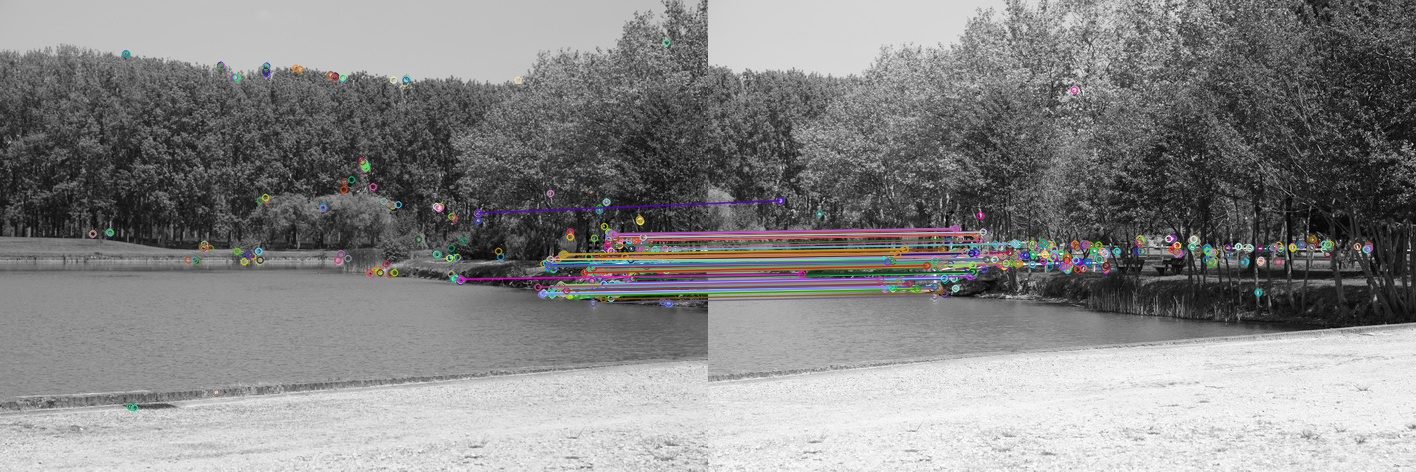
\includegraphics[width=.8\textwidth]{../resources/matchers/orb.jpg}
\captionof{figure}{Matching en utilisant ORB}
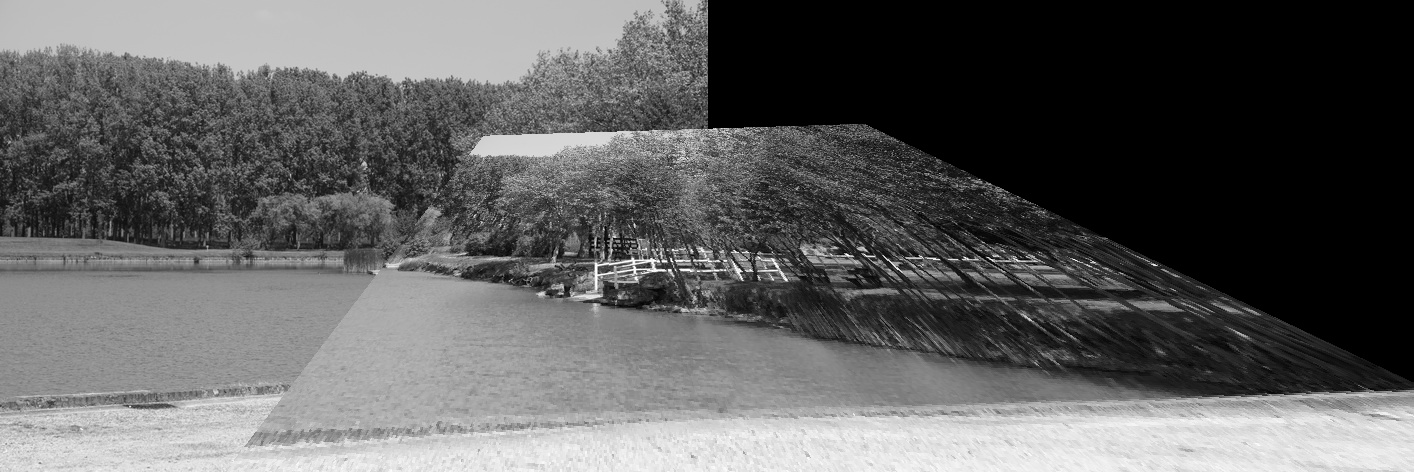
\includegraphics[width=.8\textwidth]{../resources/matchers/orb_pano.jpg}
\captionof{figure}{Le pano résultant en utilisant ORB}
\end{figure}

\begin{figure}[H]
\centering
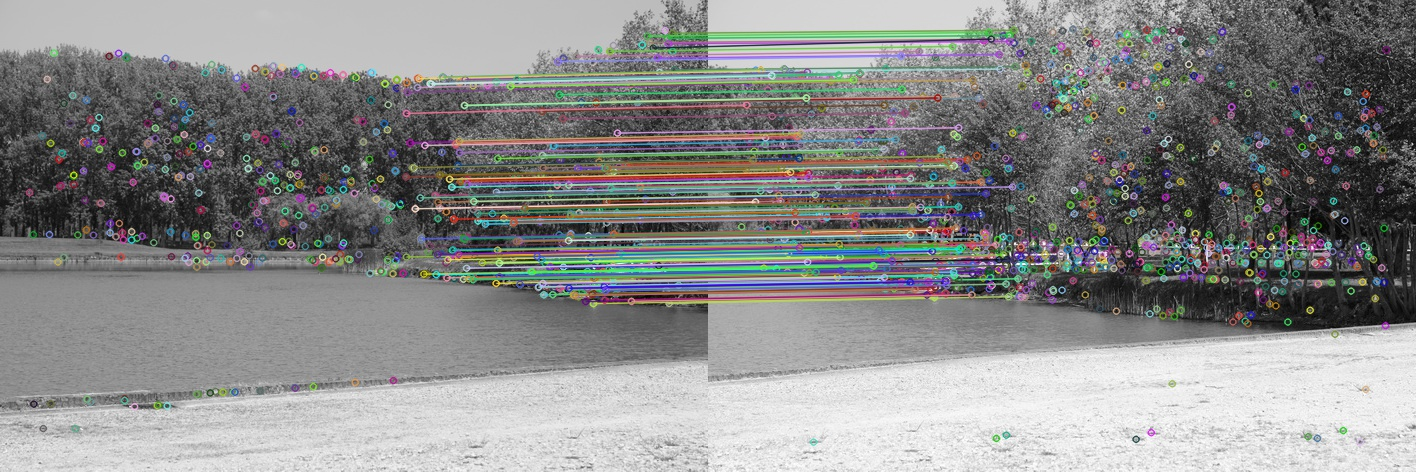
\includegraphics[width=.8\textwidth]{../resources/matchers/akaze.jpg}
\captionof{figure}{Matching en utilisant AKAZE}
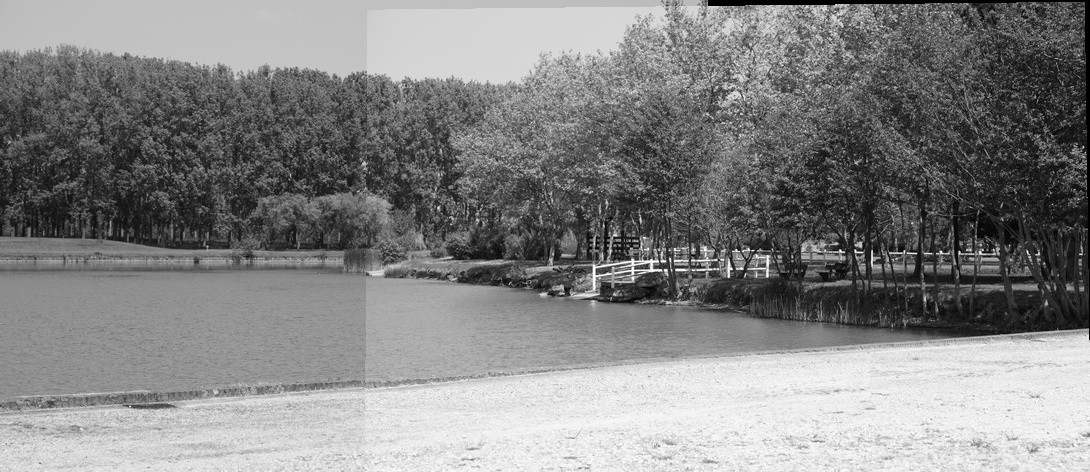
\includegraphics[width=.8\textwidth]{../resources/matchers/akaze_pano.jpg}
\captionof{figure}{Le pano résultant en utilisant AKAZE}
\end{figure}

Une autre différence qu’on a vu c’est que notre algorithme étaient beaucoup plus lent que findHomography(). En analysant plus précisément on a réalisé que c’était dû au nombre d'itération. FindHomography() pouvait trouver un bonne homographie en 100 iteration pendant que nous on trouvait pas et devait faire plutôt 2000-3000 iteration. Pour améliorer cela on donc essayé en améliorant notre RANSAC. Au lieu de retourner l'homographie avec plus de inliers, retourner une homographie avec un minimum de inliers et avec le moins possible d'erreur moyen. Mais cela n’a pas marché, le nombre de inlier étant un bonne mesure de la qualité du modèle. On a donc ajouté pour seulement essayé de faire l’homographie quand les points n’était pas linéaires et c’est là que le nombre iteration nécesaires pour trouver un bon résultat c'est réduit beaucoup.

\section{Panorama}

Une fois décidé que l’homographie marchait correctement avec notre RANSAC, on a passé à l’étape suivante; utiliser notre RANSAC et les homographies pour faire un panorama avec les images de l’X. L’algorithme devrait trouver une manière de relier toute les images en une seule grande image horizontal. \\
Originalement on allait faire un calcul avec les images dans n’importe quel ordre, on prenant à chaque itération la pair d’image qui a le plus de matches. Mais vu que l’utilisateur du programme qui calcule des homographie a rarement besoin de faire un panorama avec des images sans ordre, vu que normalement on prend les images dans l’ordre et sinon on peut leur donner un ordre manuellemente, donc on a décidé de faire un algorithme qui attend les images dans l’ordre de gauche à droite.  

\subsection{Premier Essai}

Notre première idée était de prendre la première image et de calculer l’homographie qui correspond de chaque image à la première. Pour faire cela on calcule tous les pair d’homographies $H_i$ que relient un image avec l’image suivante. Une fois calculé cela on peut calculer $G_i$, les homographie entre la première images et les autres images. On calcule donc itérativement $G_i = G_{i-1} \cdot H_i$. \\
On project les images une à une en utilisant ces homographies pour obtenir le panorama. On faisant cela et on obtient: 

\begin{figure}[H]
\centering
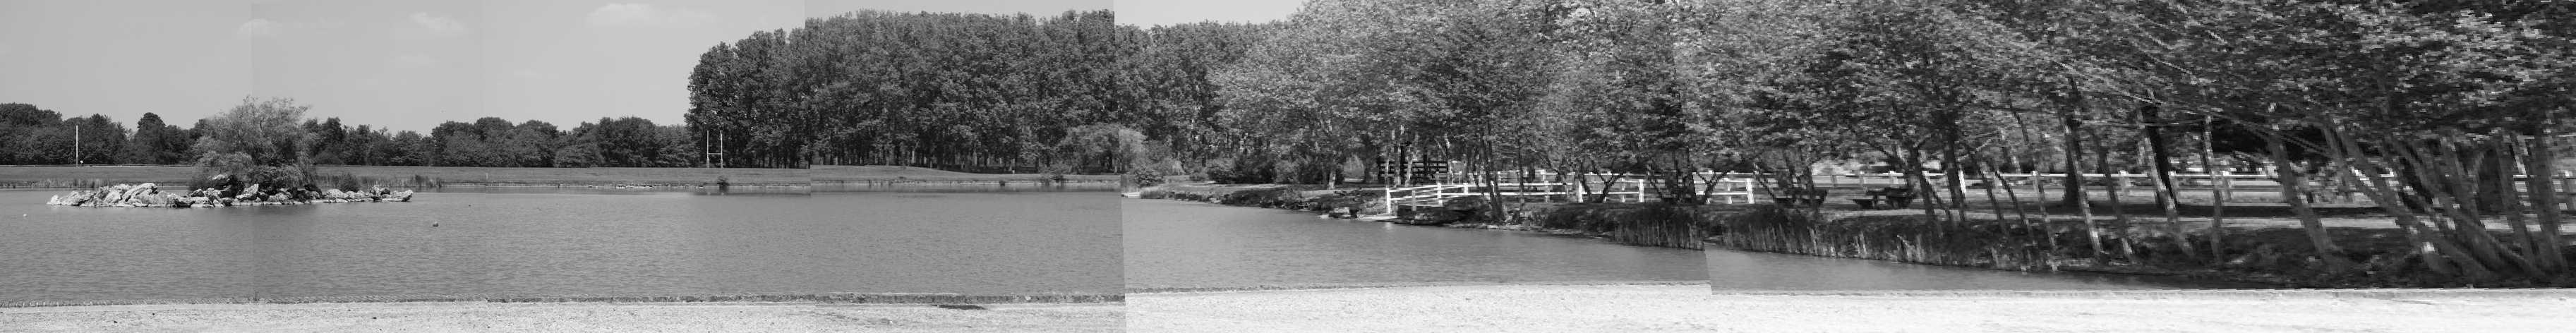
\includegraphics[width=.8\textwidth]{../resources/output/homography_panorama4.jpg}
\captionof{figure}{Le pano composé de 5 images}
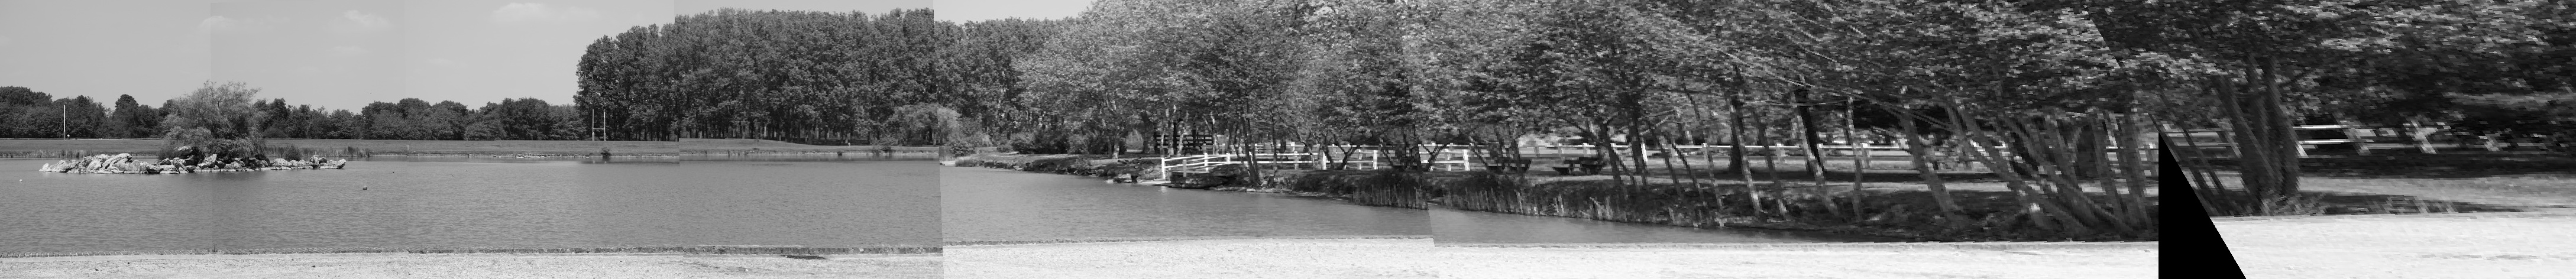
\includegraphics[width=.8\textwidth]{../resources/output/homography_panorama5.jpg}
\captionof{figure}{Le pano composé de 6 images}
\end{figure}

Comme on peut voir, les images s’étirent de plus en plus. Résultant en un panorama de plus en plus mauvais. \\
Ce qui a passé c’est comme c’est un panorama 360, à chaque étape il y a une distorsion de l’image pour projeter l’image sur l’autre, et cette distorsion et plus grande quand plus grand c’est l’angle et cet erreur s’accumule avec les successives opérations. Le résultat était donc pas bon et on pouvais faire un maximum de 4-5 images pour le panorama avant d’avoir un résultat mauvais.

\subsection{Deuxième Essai}

Pour un deuxième essai, comme on voulais réduire le problème de la distorsion à cause des grand angles de rotation, au lieu de calculer les homographie de la première image au autres on a décidé de faire un panorama auxiliaire composé des deux première images et puis itérativement calculer l’homographie entre le panorama auxiliaire et l’image suivante.

\begin{figure}[H]
\centering
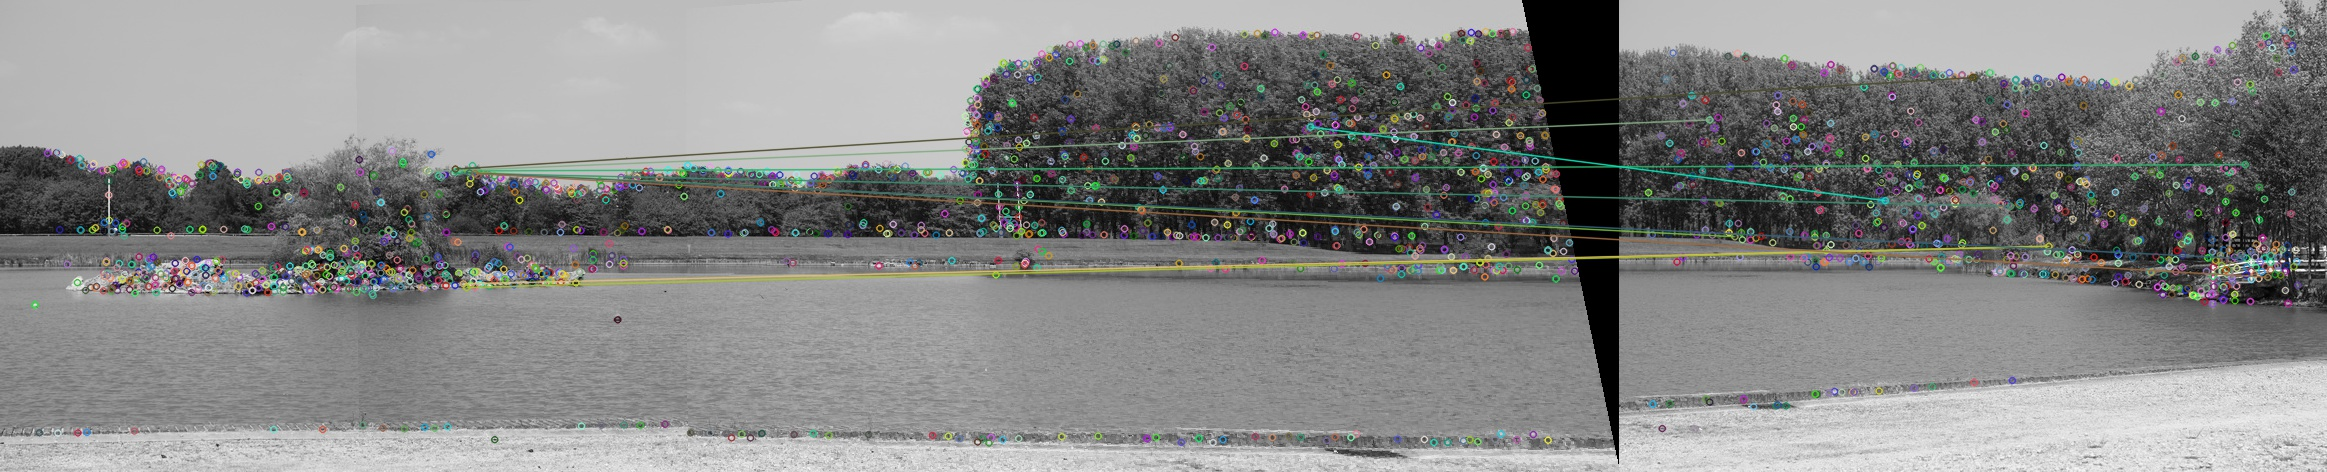
\includegraphics[width=.8\textwidth]{../resources/output/iterative_panorama2.jpg}
\captionof{figure}{Le matching en utilisant 3 images}
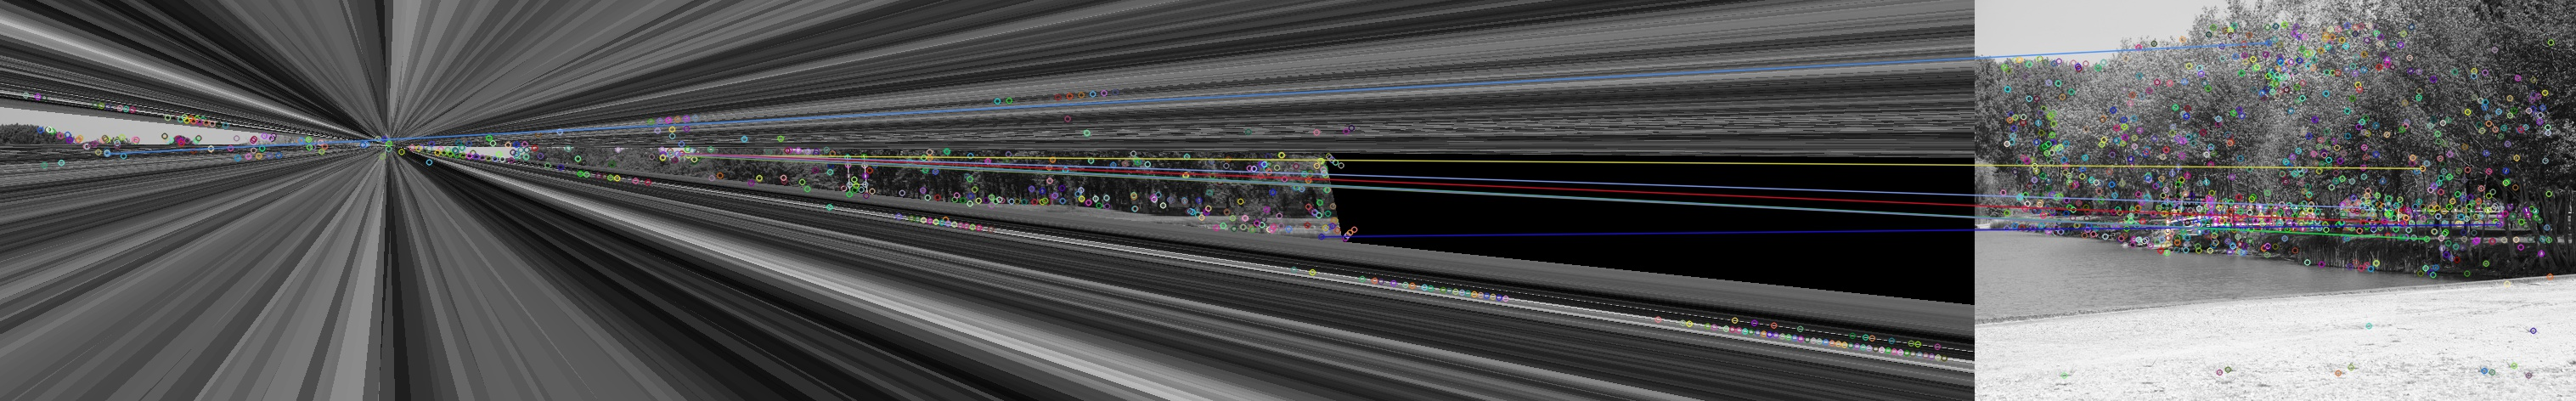
\includegraphics[width=.8\textwidth]{../resources/output/iterative_panorama3.jpg}
\captionof{figure}{Le matching en utilisant 4 images}
\end{figure}

Comme on peut voir, cet algorithme a des problèmes car à mesure que les panorama auxiliaire devient plus grand, c’est de plus en plus difficile de trouver les matches, ce qui provoque qu’en quelques itération le résultat soit complètement mauvais. \\
Mais vu que les matches peuvent être seulement entre la dernière image qui a été ajouté au panorama et la nouvelle image, et donc de la dernier partie du panorama à la nouvelle image, on a changé l’algorithme pour seulement chercher des matches entre la nouvelle images et une section du panorama auxiliaire qui avait une distance du bord plus petite que la longueur d’une image. De cet manière on chercherait seulement les matches dans la section correspondante à la dernière image, ce qui devrait réduire le nombre de mauvais matches.\\
Avec cette nouvelle condition on a obtenue ces résultats: 

\begin{figure}[H]
\centering
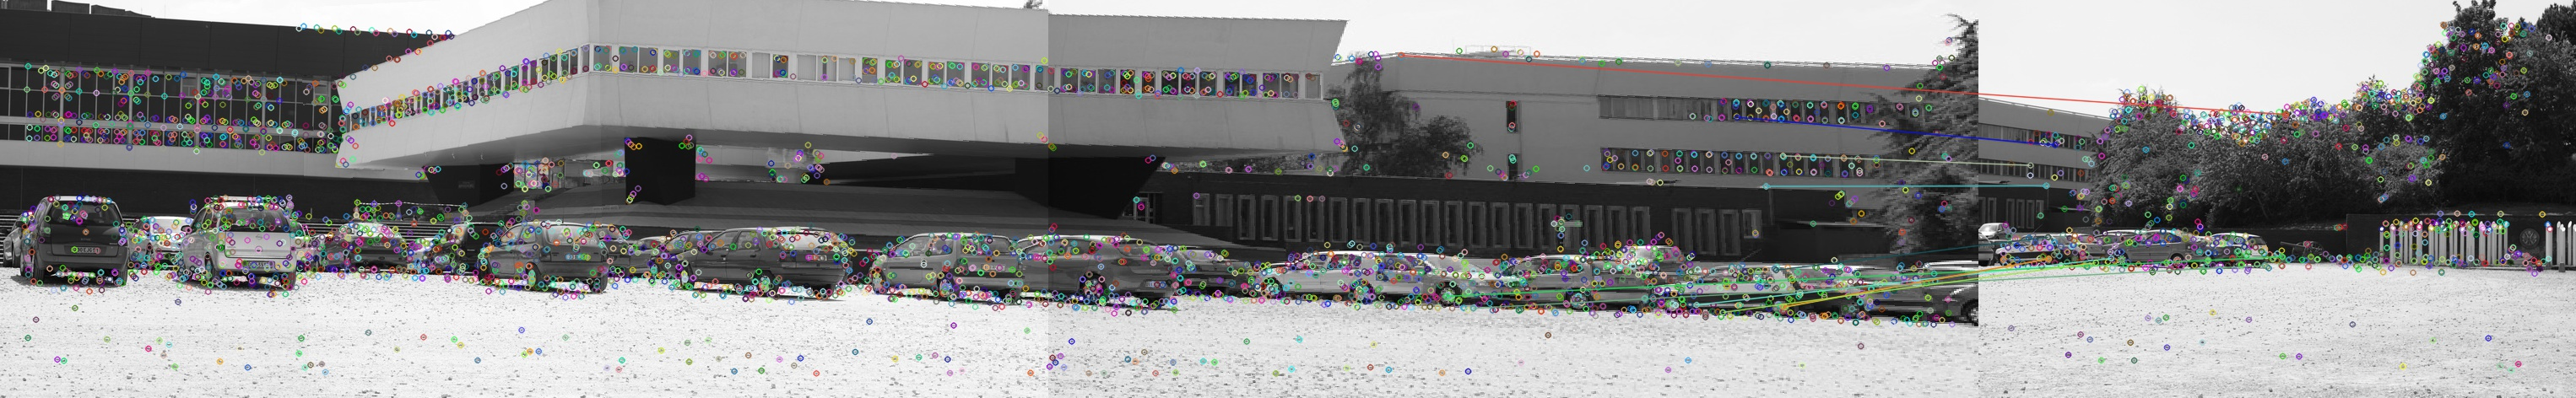
\includegraphics[width=.8\textwidth]{../resources/output/iterative_panorama_filtered3.jpg}
\captionof{figure}{Le matching en utilisant 4 images}
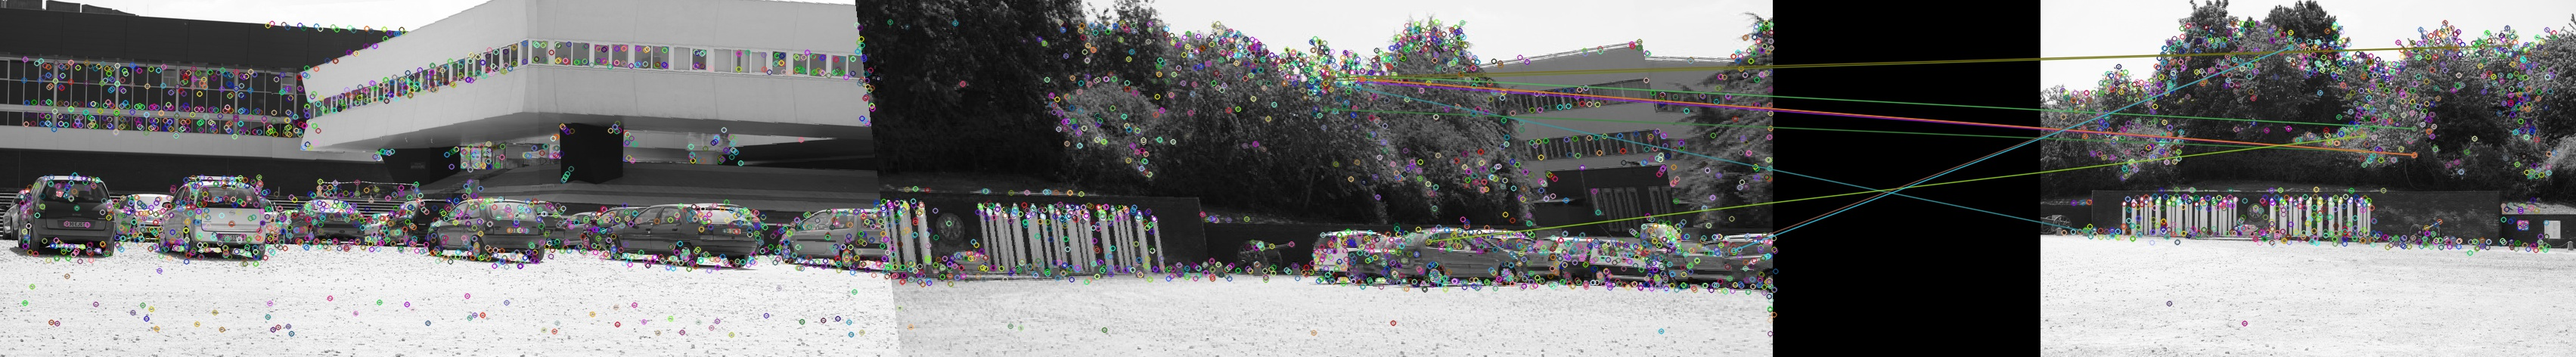
\includegraphics[width=.8\textwidth]{../resources/output/iterative_panorama_filtered4.jpg}
\captionof{figure}{Le matching en utilisant 5 images}
\end{figure}

Cela a amélioré beaucoup le résultat mais également le résultat n’est pas idéale vu que a chaque itération les nouvelles images sont de plus en plus déformé dû à leur projection et donc les matches sont de plus en plus mauvais jusqu’à que l’homographie devient fausse.

\subsection{Troisième Essai}

Vu que l’erreur était de plus en plus grand à chaque itération, on a décidé qu’au lieu d’avoir un grand panorama auquel on ajoutait des image une à une, on regrouperait les images stile arbre binaire. Cela veut dire, regroupant les images en paires pour créer des nouvelles images et itérant de cette manière jusqu’à qu’on ait une seule image. De cette manière, l’erreur dans les bord de l’image n’est pas si grand car les images sont dans une profondeur $\log(n)$ dans l’arbre, au lieu d’être à une profondeur $n$ (maximum).
Avec ce troisième essaie on a obtenue ces résultats:

\begin{figure}[H]
\centering
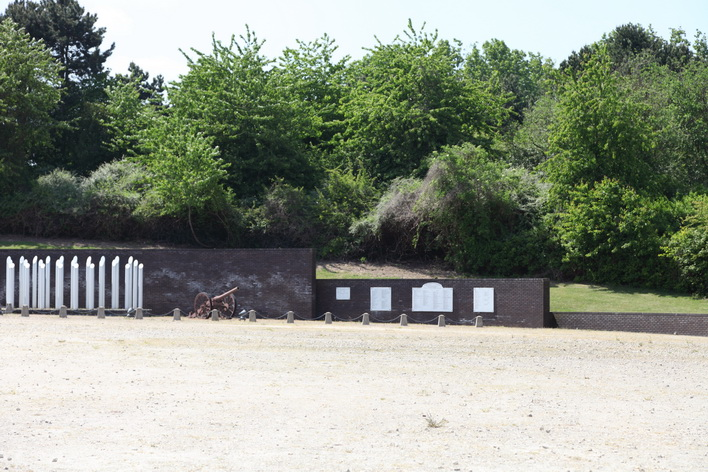
\includegraphics[width=.1\textwidth]{../resources/tour/IMG_0051.jpg}
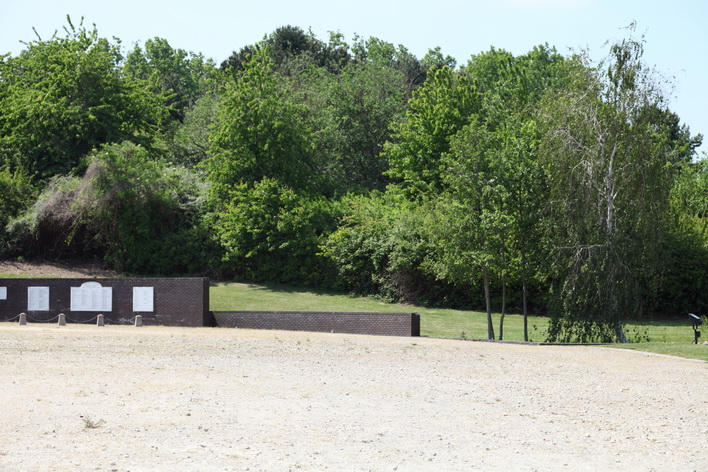
\includegraphics[width=.1\textwidth]{../resources/tour/IMG_0052.jpg}
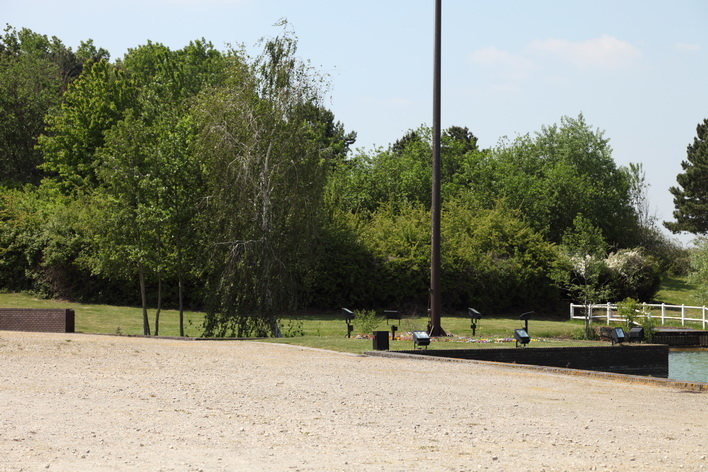
\includegraphics[width=.1\textwidth]{../resources/tour/IMG_0053.jpg}
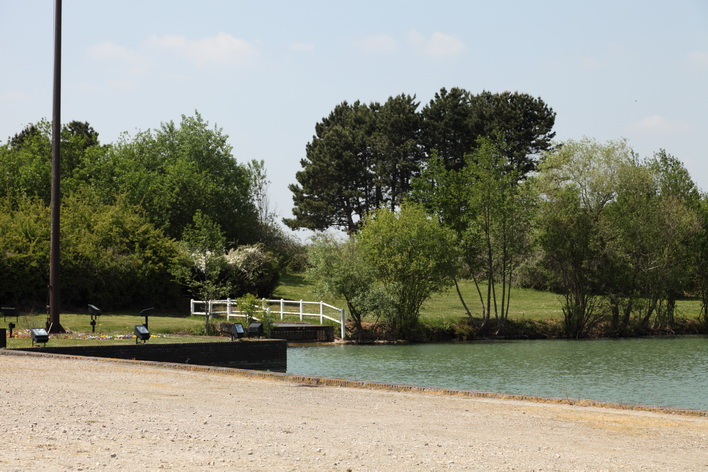
\includegraphics[width=.1\textwidth]{../resources/tour/IMG_0054.jpg}
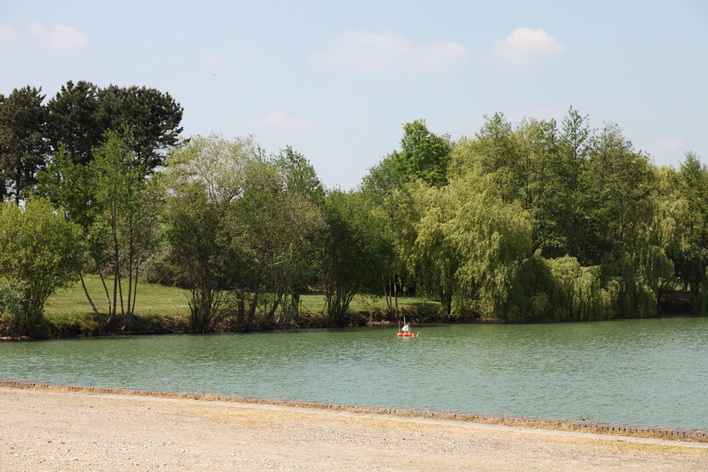
\includegraphics[width=.1\textwidth]{../resources/tour/IMG_0055.jpg}
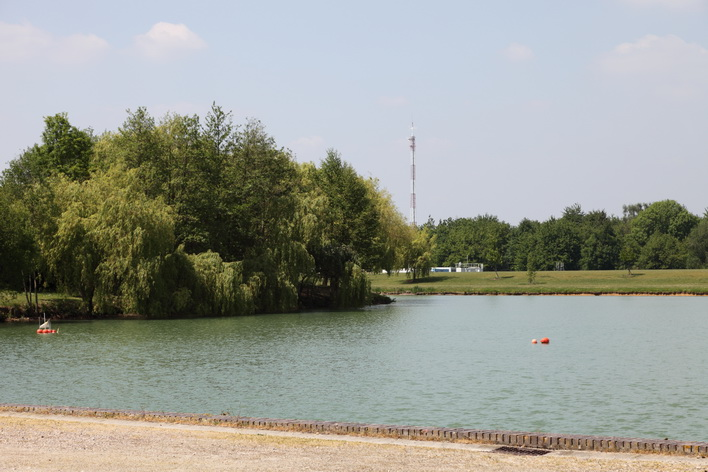
\includegraphics[width=.1\textwidth]{../resources/tour/IMG_0056.jpg}
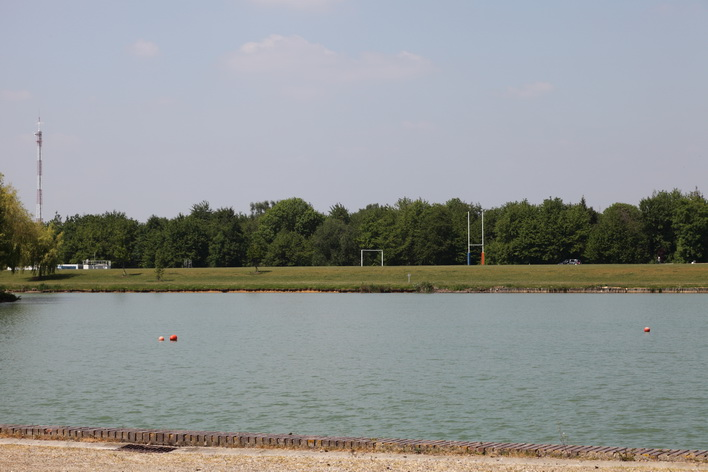
\includegraphics[width=.1\textwidth]{../resources/tour/IMG_0057.jpg}
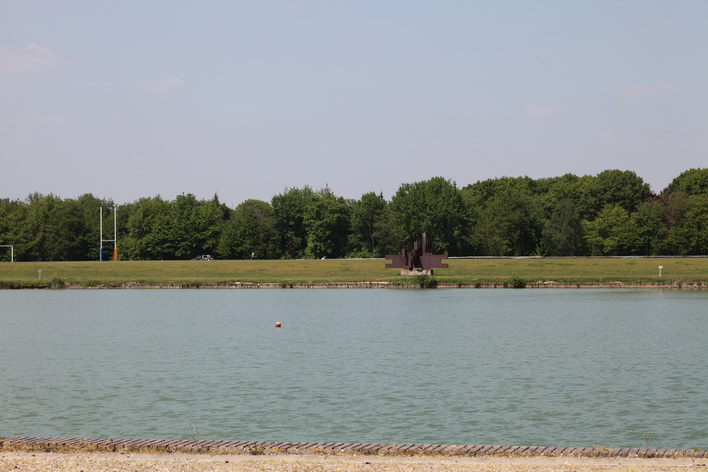
\includegraphics[width=.1\textwidth]{../resources/tour/IMG_0058.jpg}
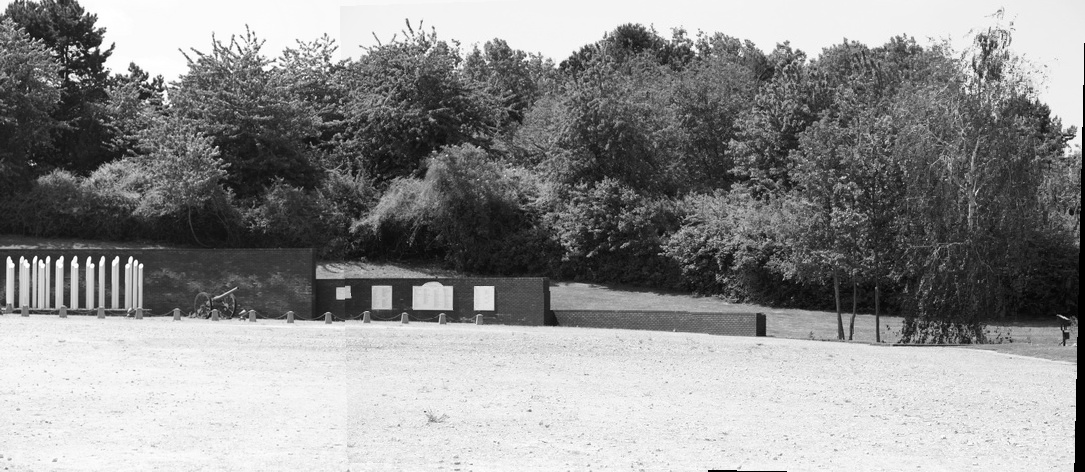
\includegraphics[width=.2\textwidth]{../resources/output/binary_panorama_selected0.jpg}
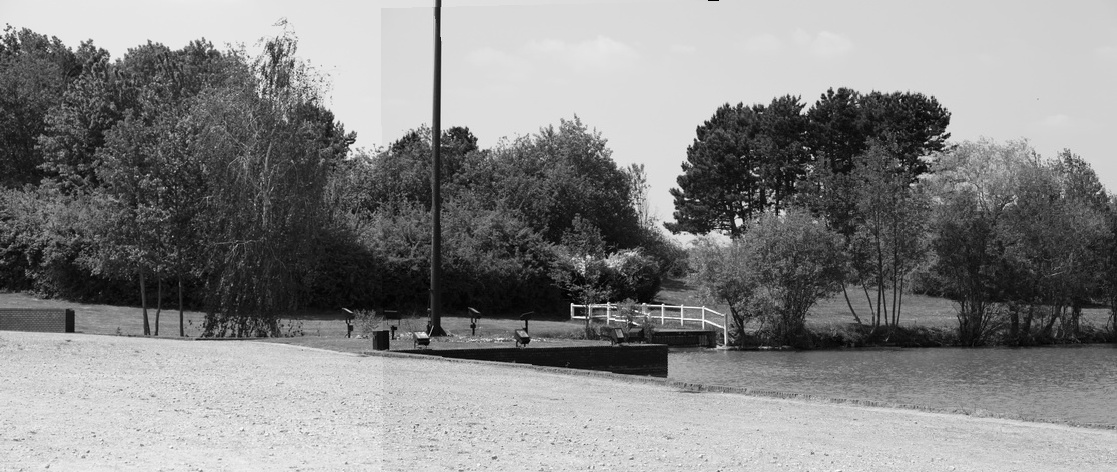
\includegraphics[width=.2\textwidth]{../resources/output/binary_panorama_selected1.jpg}
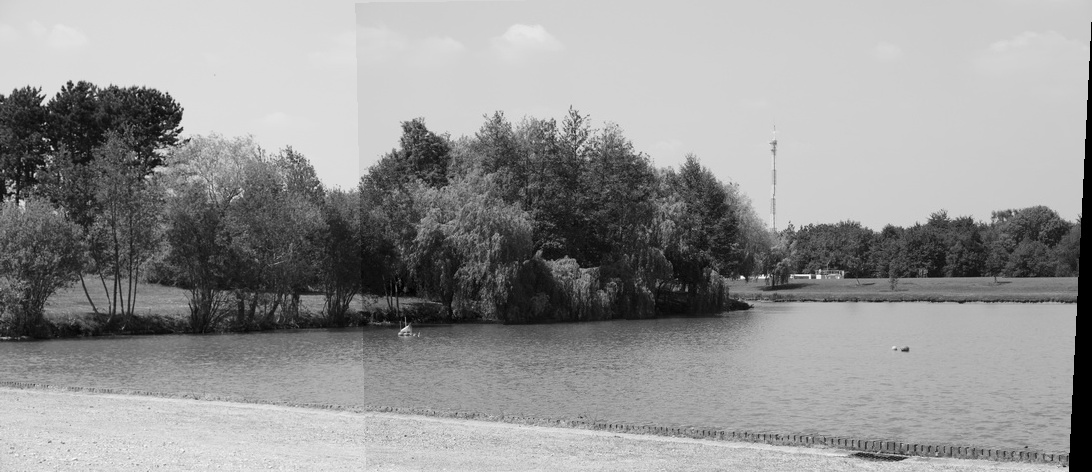
\includegraphics[width=.2\textwidth]{../resources/output/binary_panorama_selected2.jpg}
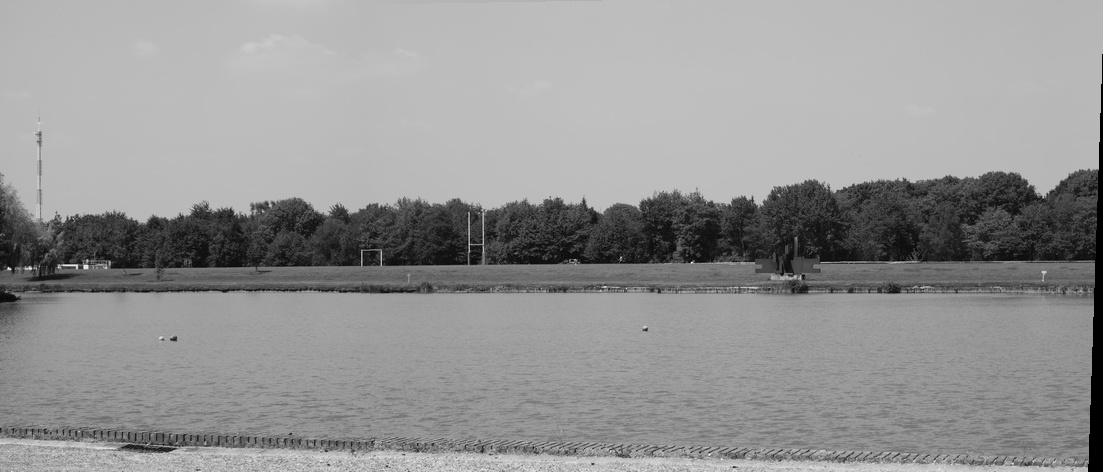
\includegraphics[width=.2\textwidth]{../resources/output/binary_panorama_selected3.jpg}
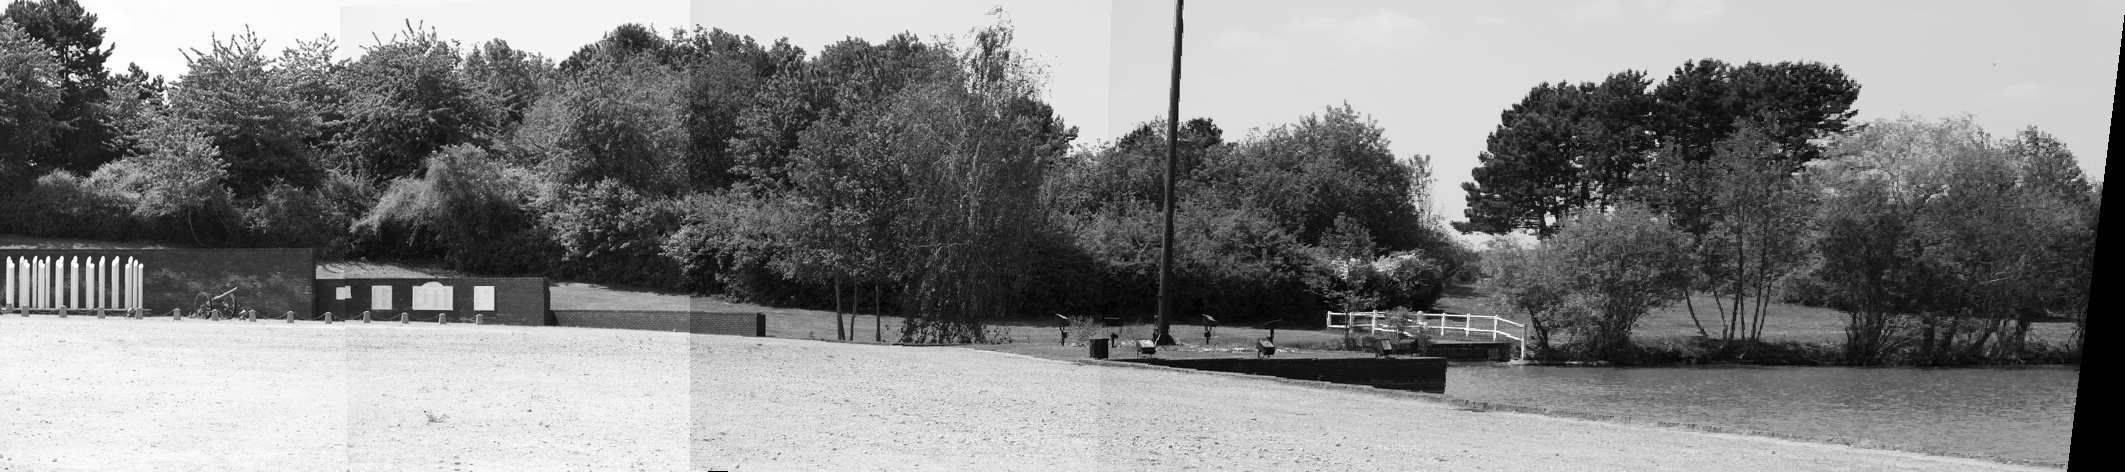
\includegraphics[width=.4\textwidth]{../resources/output/binary_panorama_selected4.jpg}
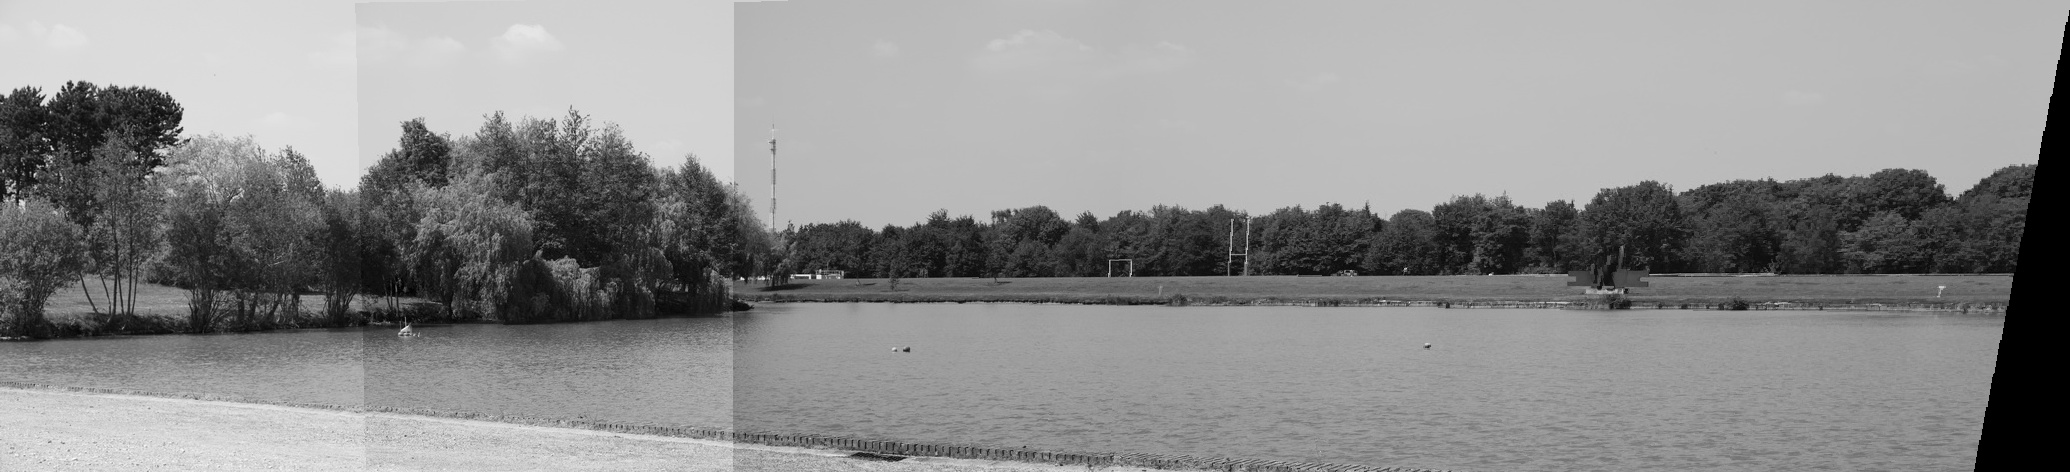
\includegraphics[width=.4\textwidth]{../resources/output/binary_panorama_selected5.jpg}
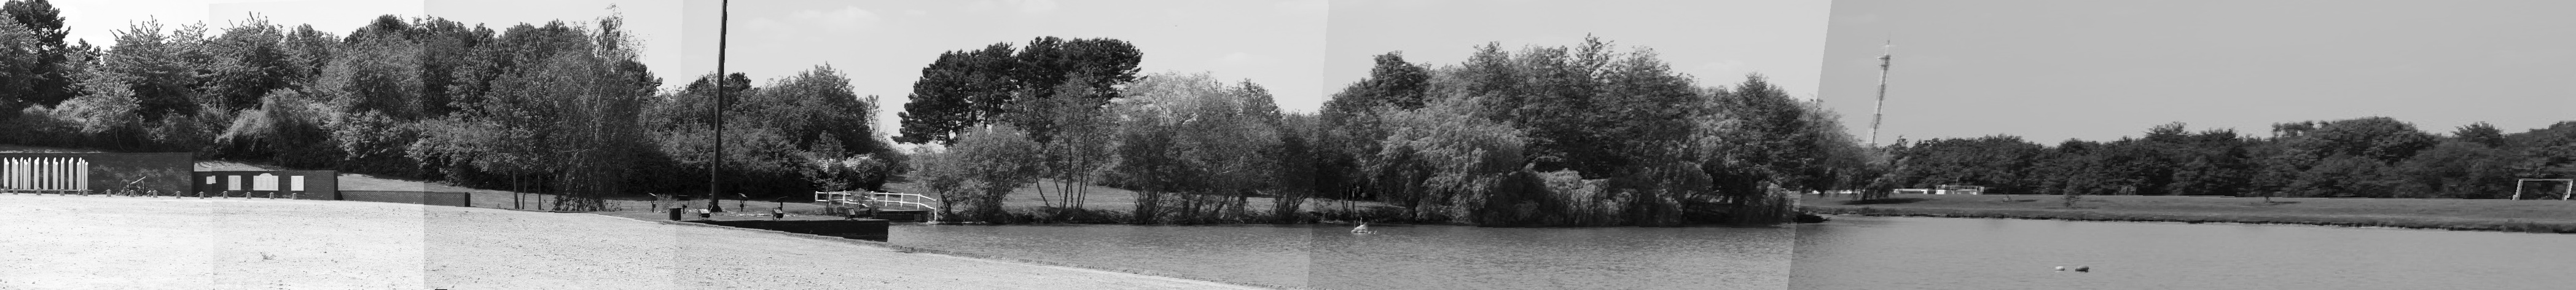
\includegraphics[width=.8\textwidth]{../resources/output/binary_panorama_selected6.jpg}
\captionof{figure}{L'algorithme binaire appliqué à 8 images}
\end{figure}

Comme on peut voir, les résultat continuent à ne pas être parfait, mais maintenant c’est pas du à un erreur accumulé mais dû au fait que quelques paires d’images ont des homographies très mauvaises, que c’est le cas de quelque images du panorama de la cour de Polytechnique où la section où quelques images se superposent est très petite.

\section{Conclusion}

L’algorithme de RANSAC est un algorithme avec une logique très simple mais très puissant, vu que celui là peut être utilisé dans n’importe quel problème où on doit trouver un modèle à partir de ensemble de donnée. Seulement on doit connaitre comment calculer le modèle à partir des donnée (et donc aussi le nombre minimum des donnée nécessaires) et comment calculer l’erreur du modèle. Et vu que ces fonctions sont normalement naturelle au problèmes, elle ne sont pas difficiles de trouver, ce qui permet avoir une rapide et facile solution au problèmes de ce type. \\
D’une autre part, on peut voir que nos panoramas fonctionnent plutôt bien, mais si et seulement si les homographies originels fonctionnait bien, ça serait intéressant d’essayer de trouver d’autre manières pour trouver les homographies et les tester pour voir si il y a une méthode qui, même si elle est plus lente, fonctionne mieux dans ces cas. \\
Et dernièrement, notre panorama ne marche que pour un panorama horizontal. Ça serait aussi très intéressant d'élargir cette algorithme pour qu’il puisse créer des panorama aussi verticalement, et puis faire des panorama sphériques.  

\pagebreak
\section*{Sources}
\begin{description}[labelindent=16pt,style=multiline,leftmargin=4cm, noitemsep]
	\item[RANSAC:] Wikipedia, \url{https://en.wikipedia.org/wiki/Random_sample_consensus}
	\item[Calculating Homography:] Per Rosengren, \url{http://www.csc.kth.se/~perrose/files/pose-init-model/node17.html}
\end{description}

\end{document}
